
\subsection*{Anàlisi de mercat VLC}
\addcontentsline{toc}{subsection}{Anàlisi de mercat VLC}

El mercat global de comunicacions de llum visible està valorat en 1.800 milions de dòlars l'any en curs i s'espera que registri un CAGR del 40,1\% durant el període de previsió, arribant als 19.300 milions de dòlars al final del període de previsió. La necessitat de transferència de dades d'alta velocitat, seguretat de dades, una imminent restricció de l'espectre de RF i diversos avantatges tecnològics sobre la tecnologia Wi-Fi impulsa principalment el mercat de la comunicació amb llum visible. A més de ser més rendible, Li-Fi té diversos avantatges respecte a la tecnologia Wi-Fi actual, com ara una velocitat de transferència de dades aproximadament 100 vegades més ràpida, una major seguretat de dades, cap interferència electromagnètica i un menor ús d'energia.


\begin{figure}[h!]
    \centering
    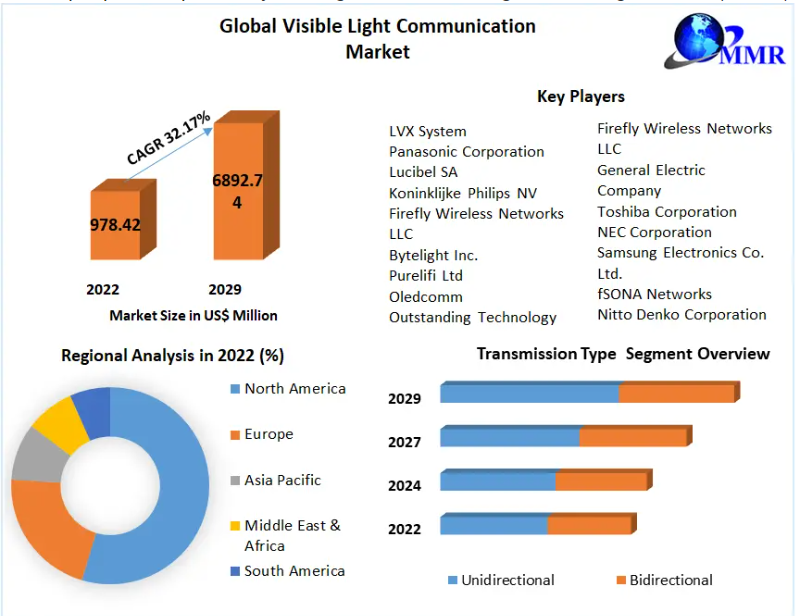
\includegraphics[width=80mm]{visiogeneralVLC.png}
    \caption{Mercat mundial del VLC }
\end{figure}



\subsection*{Tendències del mercat VLC}
\addcontentsline{toc}{subsection}{Tendències del mercat VLC}

\begin{itemize}
    \item Segons Ericsson, el nombre global de subscripcions a la xarxa mòbil de telèfons intel·ligents va superar els 6.600 milions el 2022 i s'espera que arribi als 7.800 milions el 2028. Els països amb més subscripcions a la xarxa mòbil de telèfons intel·ligents són la Xina, l'Índia i els Estats Units. Un augment tan gran dels telèfons intel·ligents crearia oportunitats lucratives per al mercat estudiat. 
    \item A més, s'esperava que les subscripcions mòbils 5G assoleixin aproximadament els 5.000 milions a finals de 2028. A més, es preveu que la cobertura de la població 5G arribi al 85\%, mentre que les xarxes 5G probablement portaran al voltant del 70\% del trànsit mòbil per al 2028. És probable que aquests esdeveniments també impulsin la demanda d'electrònica de consum, impulsant així el creixement del mercat estudiat. 
    \item Finalment, la popularitat dels dispositius domèstics intel·ligents està augmentant a mesura que els consumidors busquen maneres de fer que les seves cases siguin més còmodes, còmodes i segures. VLC pot controlar dispositius domèstics intel·ligents, cosa que la converteix en una tecnologia clau per al mercat.
\end{itemize}


\begin{figure}[h!]
    \centering
    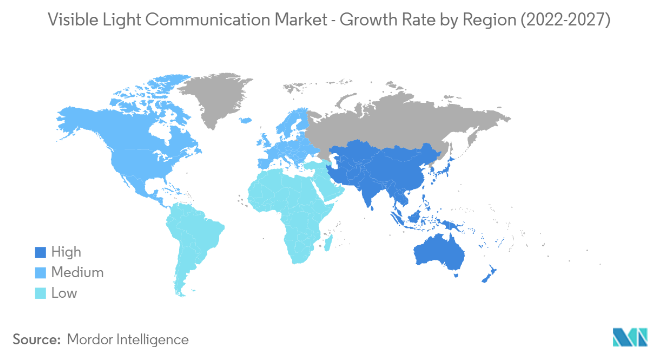
\includegraphics[width=100mm]{futurMundial.png}
    \caption{Amèrica del Nord comptarà amb la quota de mercat més gran}
\end{figure}








